%
% buchcover.tex -- Cover für das Buch Numerik
%
% (c) 2018 Prof Dr Andreas Müller, Hochschule Rapperswil
%
\documentclass[11pt]{standalone}
\usepackage{tikz}
\usepackage{times}
\usepackage{geometry}
\usepackage{german}
\usepackage[utf8]{inputenc}
\usepackage[T1]{fontenc}
\usepackage{times}
\usepackage{amsmath,amscd}
\usepackage{amssymb}
\usepackage{amsfonts}
\usepackage{txfonts}
\usepackage{ifthen}
\usetikzlibrary{math}
\geometry{papersize={402mm,278mm},total={405mm,278mm},top=72.27pt, bottom=0pt, left=72.27pt, right=0pt}
\newboolean{guidelines}
\setboolean{guidelines}{true}
%\setboolean{guidelines}{false}

\begin{document}
\begin{tikzpicture}[>=latex, scale=1]
\tikzmath{
	real \ruecken, \einschlag, \gelenk, \breite, \hoehe;
	\ruecken = 2.5;
	\einschlag = 1.6;
	\gelenk = 0.7;
	\breite = 16.7;
	\hoehe = 24.6;
	real \bogengreite, \bogenhoehe;
	\bogenbreite = 2 * (\breite + \einschlag + \gelenk) + \ruecken;
	\bogenhoehe = 2 * \einschlag + \hoehe;
}

%\clip (0,0) circle (6);

\draw[fill=blue](0,0) rectangle({\bogenbreite},{\bogenhoehe});
\hsize=13.6cm

\begin{scope}
\clip (0,0) rectangle({\bogenbreite},{\bogenhoehe});
\node at (20.7,9.0) [scale=4.5]{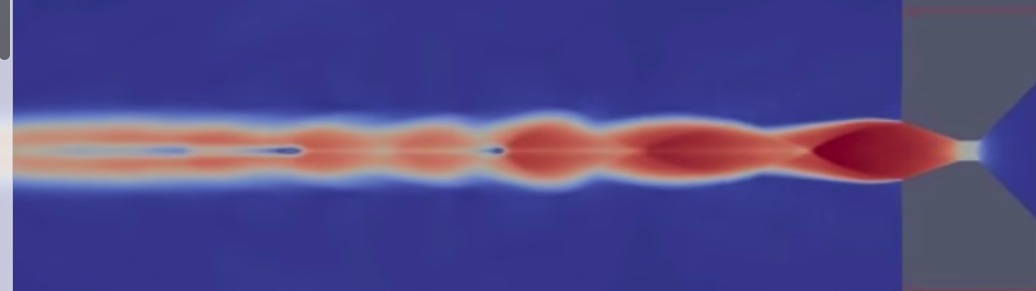
\includegraphics{nozzle.jpg}};
\end{scope}

\node at ({\einschlag+2*\gelenk+\ruecken+1.5*\breite},24.3)
	[color=white,scale=1]
	{\hbox to\hsize{\hfill%
	\sf \fontsize{24}{24}\selectfont Mathematisches Seminar}};

\node at ({\einschlag+2*\gelenk+\ruecken+1.5*\breite},21.9)
	[color=white,scale=1]
	{\hbox to\hsize{\hfill%
	\sf \fontsize{50}{50}\selectfont Numerik}};

\node at ({\einschlag+2*\gelenk+\ruecken+1.5*\breite},19.7)
	[color=white,scale=1]
	{\hbox to\hsize{\hfill%
	\sf \fontsize{13}{5}\selectfont Andreas Müller}};

\node at ({\einschlag+2*\gelenk+\ruecken+1.5*\breite},18.4)
	[color=white,scale=1]
	{\hbox to\hsize{\hfill%
	\sf \fontsize{13}{5}\selectfont
	Benjamin Bouhafs-Keller,	% B
	Daniel Bucher, 			% I
	Manuel Cattaneo%,		% E
	}};

\node at ({\einschlag+2*\gelenk+\ruecken+1.5*\breite},17.75)
	[color=white,scale=1]
	{\hbox to\hsize{\hfill%
	\sf \fontsize{13}{5}\selectfont
	Patrick Elsener,		% MSE
	Reto Fritsche,			% E
	Niccolò Galliani,		% E
	Tobias Grab%,			% MSE
	}};

\node at ({\einschlag+2*\gelenk+\ruecken+1.5*\breite},17.1)
	[color=white,scale=1]
	{\hbox to\hsize{\hfill%
	\sf \fontsize{13}{5}\selectfont
	%Rahel Hertelendy,		% B
	Thomas Kistler,			% I
	%Marc Kühne,			% B
	Fabio Marti,			% E
	Joël Rechsteiner,		% E
	Cédric Renda%,			% E (2)
	}};
 
\node at ({\einschlag+2*\gelenk+\ruecken+1.5*\breite},16.45)
	[color=white,scale=1]
	{\hbox to\hsize{\hfill%
	\sf \fontsize{13}{5}\selectfont
	Michael Schmid,		% E (2)
	Mike Schmid,			% I
	Michael Schneeberger,		% E
	Martin Stypinski%,		% IFS
	}};

\node at ({\einschlag+2*\gelenk+\ruecken+1.5*\breite},15.8)
	[color=white,scale=1]
	{\hbox to\hsize{\hfill%
	\sf \fontsize{13}{5}\selectfont
	Manuel Tischhauser,		% E (2)
	Nicolas Tobler,			% MSE
	Raphael Unterer,		% MSE
	Severin Weiss%,			% EEU
	}};

\node at ({\einschlag+2*\gelenk+\ruecken+1.5*\breite},15.15)
	[color=white,scale=1]
	{\hbox to\hsize{\hfill%
	\sf \fontsize{13}{5}\selectfont
	%Reto Wildhaber%			% B
	}};
 
%\node at (0,3) [color=white] {\sf \LARGE Mathematisches Seminar 2017};

% Rücken
\node at ({\bogenbreite/2 + 0.05},20.5) [color=white,rotate=-90]
	{\sf\fontsize{35}{0}\selectfont Numerik};

% Buchrückseite
\node at ({\einschlag+0.5*\breite},18.6) [color=white] {\sf
\fontsize{13}{16}\selectfont
\vbox{%
\parindent=0pt
%\raggedright
Im Rahmen des Mathematischen Seminars der Hochschule für Technik Rapperswil
wurden im Frühjahrssemester 2020 das Thema Numerik behandelt.
Dieses Buch bringt das Skript des Vorlesungsteils mit den von den
Seminarteilnehmern beigetragenen Seminararbeiten zusammen.
}};


\ifthenelse{\boolean{guidelines}}{
\draw[white] (0,{\einschlag})--({\bogenbreite},{\einschlag});
\draw[white] (0,{\bogenhoehe-\einschlag})--({\bogenbreite},{\bogenhoehe-\einschlag});

\draw[white] ({\einschlag},0)--({\einschlag},{\bogenhoehe});
\draw[white] ({\einschlag+\breite},0)--({\einschlag+\breite},{\bogenhoehe});
\draw[white] ({\einschlag+\breite+\gelenk},0)--({\einschlag+\breite+\gelenk},{\bogenhoehe});
\draw[white] ({\bogenbreite-\einschlag-\breite-\gelenk},0)--({\bogenbreite-\einschlag-\breite-\gelenk},{\bogenhoehe});
\draw[white] ({\bogenbreite-\einschlag-\breite},0)--({\bogenbreite-\einschlag-\breite},{\bogenhoehe});
\draw[white] ({\bogenbreite-\einschlag},0)--({\bogenbreite-\einschlag},{\bogenhoehe});
}{}

\end{tikzpicture}
\end{document}
